\documentclass[12pt]{article}
\usepackage{german}
\usepackage{todonotes}
\usepackage{tikz}
\usepackage[utf8]{inputenc}
\usepackage{adjustbox}
\usepackage{graphicx}
\usepackage{afterpage}
\usepackage{listings}
\usepackage{float}
\graphicspath{{./images/}}
\lstset{language=Python}

\begin{document}

%\listoftodos
\tableofcontents
\newpage

\part{Erianet}
\section{Einleitung}
%\todo{Namensherkunft}
\paragraph{}
Das Erianet ist eine mit Python entwickelte Software, die
durch ein Neurales Netzwerk f"ahig ist,
Personen anhand ihrer Gesichter unterscheiden.
Es wurde von Mayrhofer Erik und Schwarcz Florian
entwickelt und durch Kombination beider Vornamen und \glqq neural net\grqq{}
auf seinen Namen getauft.
%\todo{Warum Projekt?}
\paragraph{}
Im Rahmen des Schulunterrichts im Fach \glqq Systemplanung und Projektentwicklung\grqq{}
war es die Aufgabe des Projektteams, eine zur Gesichtserkennung
f"ahige Software zu entwickeln.
%\todo{Welche Technologien}
Bei der Entwicklung bediente man sich einiger Python-Libraries.
So wurde OpenCV als Gesichtsdetektor eingesetzt und mit Keras das neurale
Netz erstellt und trainiert.
\paragraph{}
Zum Trainieren des Modells wurden vorgefertigte Sammlungen f"ur genau diesen
Zweck auf dem Internet verwendet. Einige davon waren die \glqq Labelled Faces in the Wild\grqq{},
\glqq AT\&T Faces\grqq{} und \glqq YouTube face database\grqq{}. Es wurden
auch selbst Bilder mit einem dazu erstellten Programm geschossen und zum Training verwendet.
\newpage
\section{Architektur}
\afterpage{\clearpage}
\begin{figure}[H]
    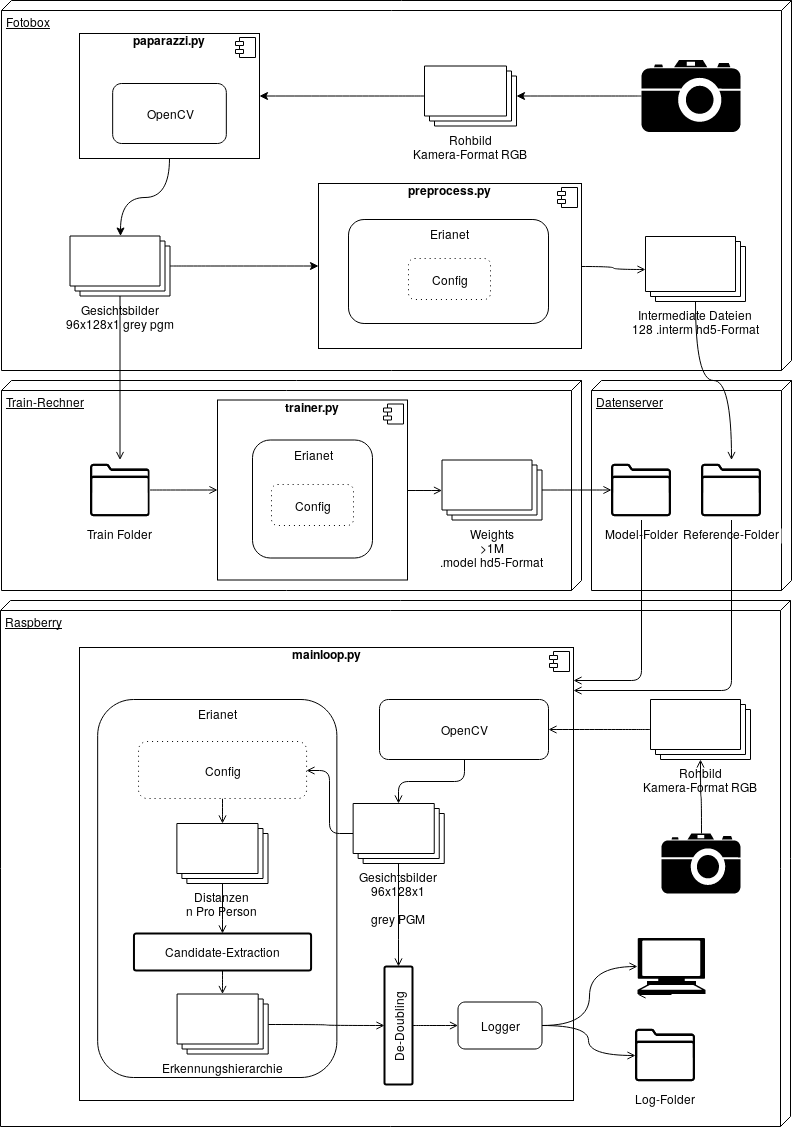
\includegraphics[height=0.9\textheight]{Architektur}
    \caption{Architektur}
\end{figure}

\subsection{Fotobox}
Die Fotobox ist ein kleiner Rechner,
mit dessen Hilfe Referenzbilder aufgenommen werden
k"onnen.
\paragraph{paparazzi.py}
greift den Kamera-Feed einer Webcam ab und nutzt
OpenCVs Haar-Classifier dazu, ein erkanntes Gesicht 
herauszuschneiden. Dieses wird dann in unser verwendetes
Format (Siehe \ref{formats}) umgewandelt.
\paragraph{preprozess.py}
nimmt die, vorher aufgenommenen Bilder und lässt sie einmal 
durch einen Fuß (Siehe \ref{neuralfoot}) des Erianet laufen. Dadurch
werden sie in die interne Repräsentation des neuralen Netzes 
umgewandelt und als sogenannte intermediate-Datei gespeichert.
Dieser Schritt spart extrem viel Rechenzeit, da sonst
jedes einzelne Bild zur Laufzeit wieder und wieder 
umgewandelt werden müsste.
\subsection{Train-Rechner}
Der Train-Rechner ist ein leistungsfähiger Rechner, welcher nur selten
benötigt wird. Damit das neurale Netz fähig wird, Gesichter verlässlich
zu unterscheiden, muss man es trainieren. Das heißt, man muss ihm viele
Daten geben, mit deren Hilfe es lernt, die vorgegebene Aufgabe zu erfüllen.
\paragraph{Train Folder} Am Train-Rechner müssen die rohen
Bilder vorhanden sein, welche vorher aufgenommen wurden.
Diese Bilder müssen nicht zwingend Bilder von Menschen sein,
die man später erkennen möchte, sondern eine möglichst diverse
Menge an unterschiedlichen Bildern von Gesichtern. Um gute Ergebnisse
zu erzielen, rechnen wir damit, eine ungefähre Menge von insgesamt
10.000 Bildern von mindestens 500 Personen zu benötigen.
\paragraph{trainer.py}
Der Trainer nutzt die Referenzdaten aus dem Train Folder 
um die weights des neuralen Netzes zu ermitteln und diese
als trainiertes Modell zu speichern.
\subsection{Raspberry}
Am Raspberry-PI würde die finale Gesichtserkennung stattfinden.
Dazu sind ein trainiertes Modell und die intermediate-Daten vonnöten.
\paragraph{mainloop.py}
% TODO Fill this in
Die Mainloop ist das Hauptprogramm, das mithilfe des Erianet und einer Kamera
die aufgenommenen Gesichter erkennt und mitloggt.
\subparagraph{Erianet}
Das Erianet im Mainloop wandelt ein aufgenommenes Gesichtsbild in
das Intermediate-Format um und vergleicht dieses über die 
euklid'sche Distanz mit den Referenzbildern aus dem Reference-Folder.
Für jede Referenzklasse wird dann die durchschnittliche Distanz
ermittelt und nach dieser werden die Klassen geordnet und als
Kandidaten wieder zurückgegeben.
\paragraph{Log-Folder}
Im Log-Verzeichnis wird in einer Textdatei jede Erkennung mitprotokolliert.
Sowohl die Zeit der Erkennung als auch der Name werden gespeichert und zu
jedem Eintritt wird das Bild der Person in den Pictures-Ordner gespeichert
und nach dem Logeintrag benannt.
\subsection{Formate}
\paragraph{Kamerarohbilder}
dürfen so groß sein, wie die Kamera liefert, und müssen RGB sein.
\paragraph{Gesichtsbilder}
sind 128 Pixel hoch und 96 Pixel breit und sollten in Greyscale 
sein.
\paragraph{Intermediate}
sind im HDF5-Format gespeichert und 128 floats lang.
\paragraph{Weights}
werden von Keras gespeichert, sind im HDF5-Format. 
\label{formats}

%\todo{Diagramm mit Annotationen}
%\todo{Kapitel f"ur alle Annotationen}
\pagebreak
\section{Neurales Netz}
Als erianet.py wird in dieser Software eine Wrapper-Klasse für 
Keras bezeichnet. Diese Klasse repräsentiert eine Instanz des 
Erianet und bietet verschiedene Methoden an, welche die 
Bedienung um einiges einfacher machen. Der durchschnittliche
Lebenszyklus eines Erianet sieht folgendermaßen aus:
\begin{lstlisting}[frame=single]
net = Erianet("model.name", config=VGG19ish)

names = net.predict(image, reference_set)

for name in names:
    print(PredictResult.name(name), 
    PredictResult.difference(name))
\end{lstlisting}
In der Config sind die eigentlichen Layer des Neuralen Netzes definiert.
\subsection{Aufbau}
\label{neuralfoot}
Das Erianet baut auf einem sogenannten "Siamesischen Netzwerk" auf.
Ein siamesisches Netzwerk zeichent sich dadurch aus, dass es zwei
\glqq{}F"uße\grqq gibt, welche aus dem exakt gleichen Convolutional-Netzwerk 
bestehen, welche sich die weights teilen. Ein Bild wird durch den
einen Fuß geschickt, das andere Bild durch den anderen Fuß.
Ein Fußnetzwerk gibt jeweils einen Vektor (Intermediate-Repräsentation)
zurück und zwischen diesen Vektoren wird dann die euklid'sche Distanz
gebildet, um festzustellen, wie ähnlich die beiden Bilder sind.
\paragraph{Fußnetzwerk}
Das Fußnetzwerk ist meist ein Deep-Convolutional-Neural-Network, was heißt
dass viele Schichten von Convolutional-Layern und Pooling-Layern genutzt werden.
Der am vielversprechendste Ansatz ist ein VGG19-Netzwerk.
\subsection{Training}
Das Training eines Siamesischen Netzwerks ist supervised. Das heißt, dass
dem Netzwerk zwei Bilder gezeigt werden, und je nachdem, ob die beiden Bilder
von derselben Person oder von unterschiedlichen Personen stammen, wird dann 
versucht die Distanz zwischen den Intermediate-Vektoren möglichst hoch, oder 
niedrig zu halten.

\part{Facepong}
\section{Einleitung}
\paragraph{}
F"ur den Tag der offenen T"ur an der HTL Leonding wurde dem Projektteam
aufgetragen, mithilfe ihrer gesammelten Erfahrung im Bereich Gesichtsdetektion
ein kleines Programm zu entwickeln, welches man den Besuchern Vorstellen kann.
Dabei kam die Idee auf, ein Spiel zu programmieren, bei dem man mit seinem Gesicht
gegen einen anderen Spieler das klassische Spiel \glqq Pong\grqq{} spielen kann.
\paragraph{}
Zus"atzlich zu OpenCV f"ur die Gesichtsdetektion wurden in diesem Teil des Projektes
die Libraries PyMunk f"ur realistische Physiksimulation und PyGame für einfache Bildausgabe
herangezogen.
\section{Aufbau und Spielweise}
\paragraph{}
Zum Spielen braucht man eine Kamera und einen Monitor bzw. Beamer. Die Kamera
wird m"oglichst mittig entweder unter oder "uber der Bildausgabe aufgestellt und angeschlossen.
Anschließend wird das Programm gestartet und es kann gespielt werden.
Betreten die beiden Spieler ihren Bereich links und rechts vor der Kamera,
startet das Spiel automatisch. Der Ball kann nun mit dem Kopf angestoßen werden
und muss das Tor des Gegners ber"uhren. Zu beachten ist hierbei, dass
das Gesicht jederzeit gerade zur Kamera gerichtet sein muss, damit es erkannt werden kann.
\section{Probleme und Zukunftspl"ane}
\paragraph{}
%\todo{Probleme und Z.}
Wie bereits erw"ahnt muss man den Kopf zu jeder Zeit gerade in Richtung
der Kamera halten. Dadurch wird bei zu großer Neigung durch nach unten oder zur
Seite blicken das Spiel angehalten, da kein Gesicht erkannt wird.
\paragraph{}
Zuk"unftige Verbesserungen w"aren zum einen die Behebung des oben genannten Problems
durch Einsatz besserer Modelle unter Beachtung der Performance. Das Spiel l"auft aktuell
in 480p und verlangsamt sich beim Upgrade auf 1080p auf unter 10 Bilder pro Sekunde,
was auf das inperformante Modell zur Gesichtsdetektion zur"uckzuf"uhren ist.
F"ur den jetzigen Einsatz mit Beamer und Kamera sind 480p jedoch ausreichend.
\section{Architektur}
%\todo{Architektur}
\end{document}